
%(BEGIN_QUESTION)
% Copyright 2006, Tony R. Kuphaldt, released under the Creative Commons Attribution License (v 1.0)
% This means you may do almost anything with this work of mine, so long as you give me proper credit

Pneumatic diaphragm and piston actuators are usually equipped with powerful springs to ensure a particular fail mode.  Take for instance this illustration for a pneumatic diaphragm actuator:

$$\includegraphics[width=8.5cm]{i00789x01.eps}$$

A series of nuts and bolts hold the upper and lower halves of the actuator together.  These same bolts hold back the spring's force, which makes them potentially dangerous to remove!  If one was to simply remove all the bolts at once, the top half of the actuator would fly off from the bottom half, possibly causing injury or equipment damage.

How, then, can we safely disassemble the actuator?  How may we relieve the tension from the large spring safely {\it before} we completely separate the top half of the actuator from the bottom half?

\vskip 20pt \vbox{\hrule \hbox{\strut \vrule{} {\bf Suggestions for Socratic discussion} \vrule} \hrule}

\begin{itemize}
\item{} Is this a {\it direct} or {\it reverse} acting actuator?
\item{} Does the spring operate in a mode of {\it tension} or of {\it compression}?
\item{} If this actuator were connected to a {\it direct-acting} control valve body, would the resulting valve assembly be {\it air-to-open} or {\it air-to-close}?
\item{} If this actuator were connected to a {\it reverse-acting} control valve body, would the resulting valve assembly be {\it fail-open} or {\it fail-close}?
\end{itemize}

\underbar{file i00789}
%(END_QUESTION)





%(BEGIN_ANSWER)

Hint: you will need to remove {\it some} of the bolts, replacing them with longer bolts, during the disassembly process!

%(END_ANSWER)





%(BEGIN_NOTES)

Remove every other bolt (half of the total number of bolts holding the actuator halves together), then replace those removed bolts with {\it longer} bolts and tighten down their nuts.  Now, remove the remaining original bolts.  Finally, begin to loosen the longer bolts previously installed.  Their additional length will give the mechanism the displacement it needs to relieve spring pressure.

\vskip 10pt

This procedure may be repeated more than once, using successively longer stages of bolts, if the spring's de-compression travel is longer than expected.


%INDEX% Final Control Elements, valve: disassembly of spring actuator

%(END_NOTES)


